\newpage

\section*{ $^{63}$Cu(n,$\gamma$)$^{64}$Cu }

Power Level: 100 kW(th) \\
Time at Power: 60.0 m \\
Wait Time:  2.0 d \\
Counting Time: 60.0 m \\
Total Activity at Removal: 3.94e+01 $\mu Ci$

\begin{table*}[h]
\centering
\begin{tabular}{ |c|c|c|c|c|c| }
 \hline
 Position & Mass $mg$ & Counting Activity $\mu Ci$ & Area (Counts) & Error \% \\
 \hline 
 1 & 1.35 & 4.87e+00 & 4.74e+04 & 0.4593 \\ 
\hline
 2 & 1.35 & 7.37e+00 & 7.17e+04 & 0.3734 \\ 
\hline
 3 & 1.35 & 6.78e+00 & 6.59e+04 & 0.3896 \\ 
\hline
 4 & 1.35 & 3.88e+00 & 3.77e+04 & 0.5148 \\ 
\hline
\end{tabular}
\end{table*}

\begin{figure}[h]
\centering
\begin{subfigure}{.5\textwidth}
  \centering
     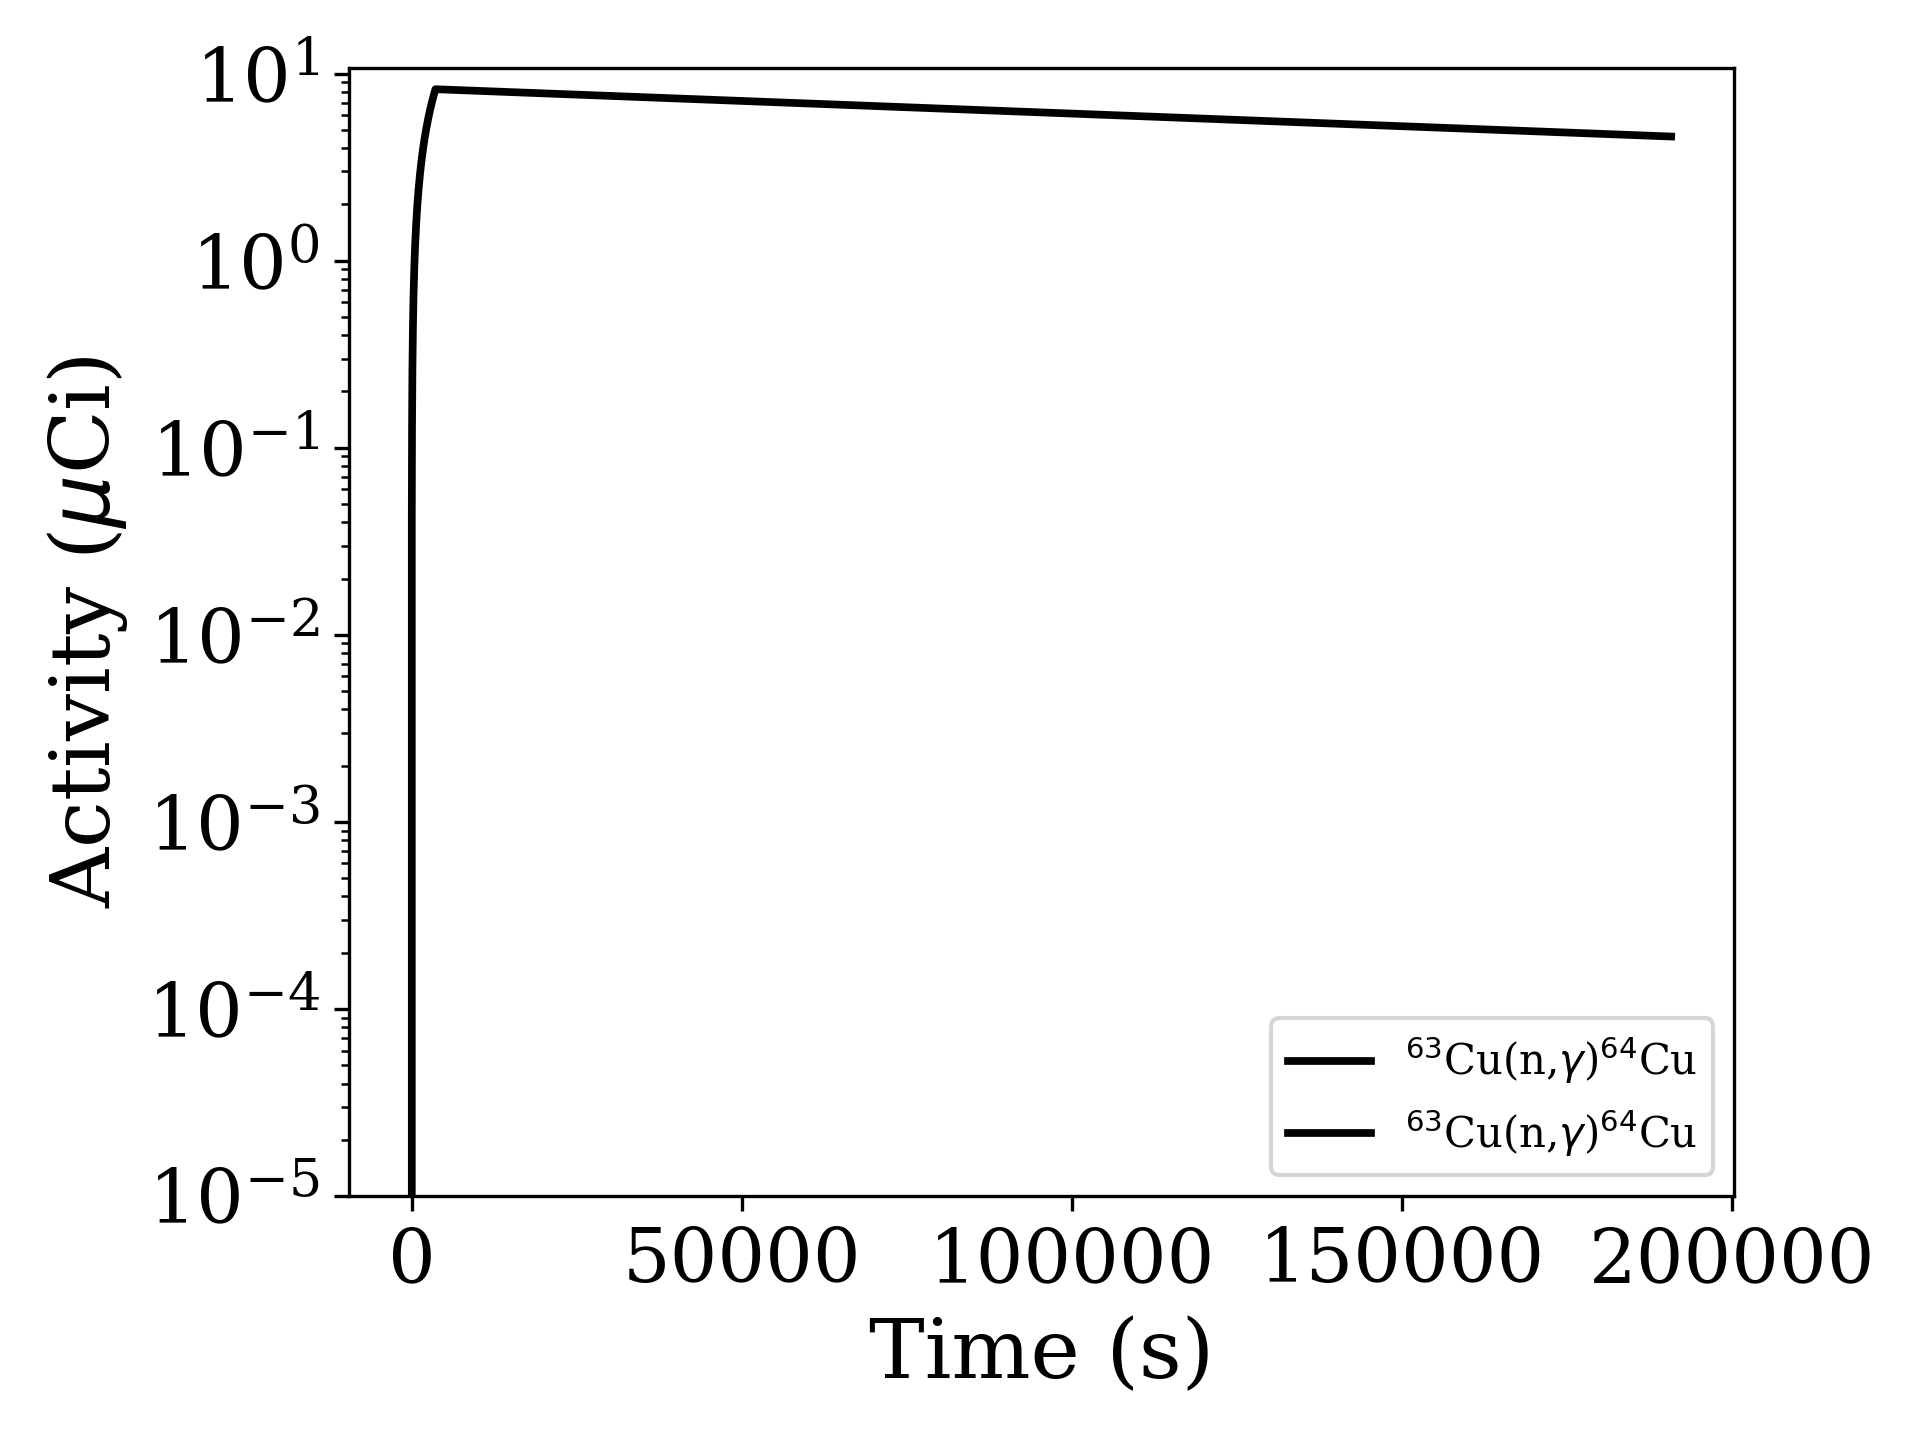
\includegraphics[width=.8\textwidth]{plot/Cu-63(n,gamma)Cu-64_library1} 

  \caption{A subfigure}
  \label{fig:sub1}
\end{subfigure}%
\begin{subfigure}{.5\textwidth}
  \centering
     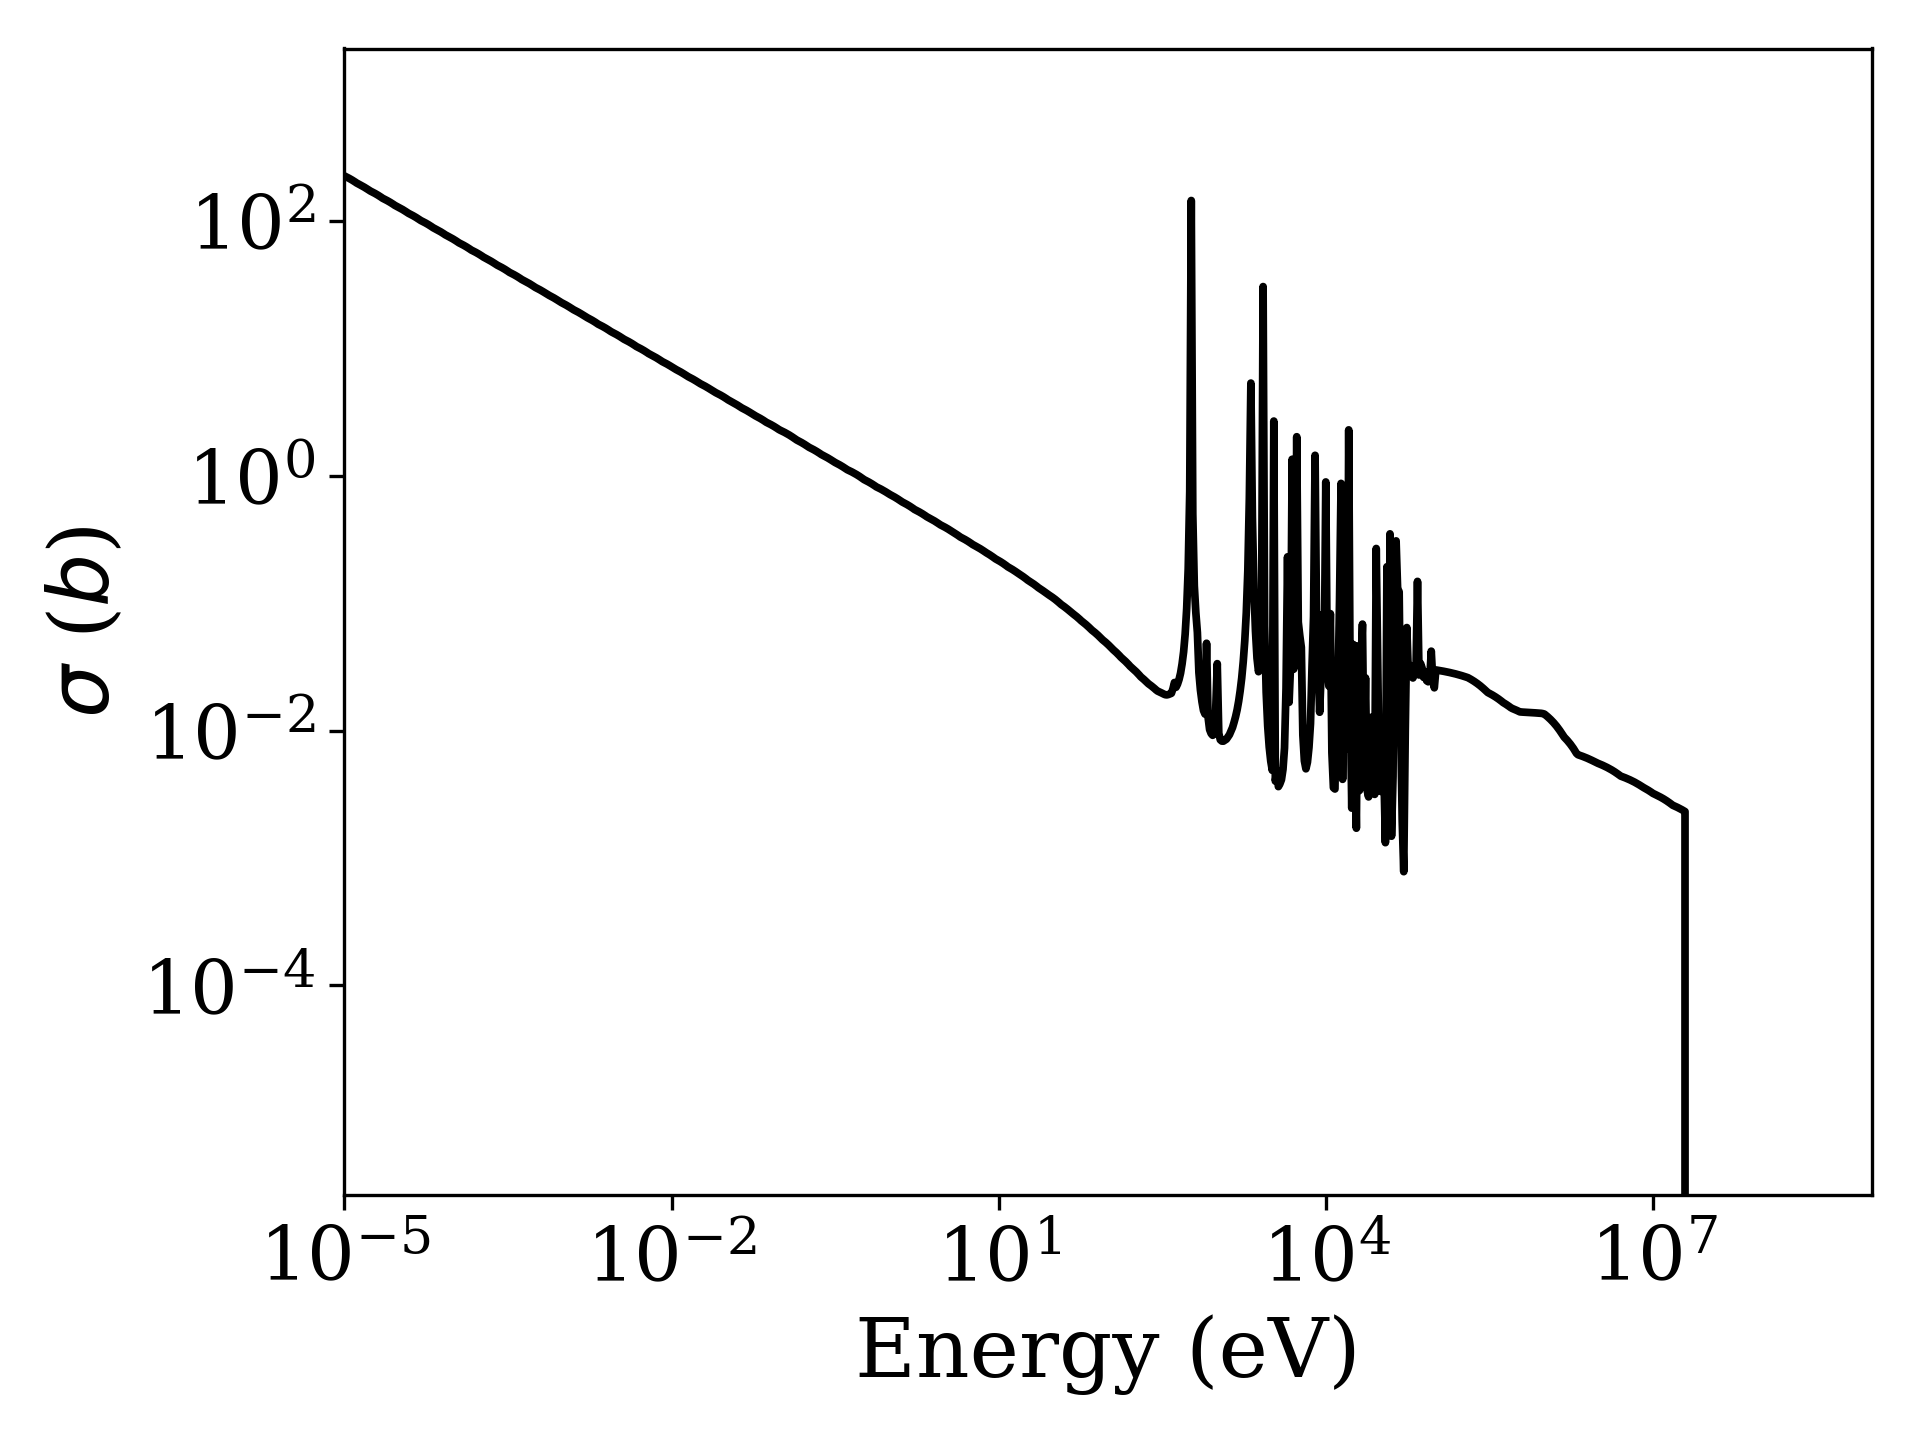
\includegraphics[width=.8\textwidth]{plot/Cu-63(n,gamma)Cu-64} 

  \caption{A subfigure}
  \label{fig:sub2}
\end{subfigure}
\caption{A figure with two subfigures}
\label{fig:test}
\end{figure}

\begin{table*}[h]
\centering
\begin{tabular}{ |c|c|c|c|c|c|c| }
 \hline
 Reaction & T$_{1/2}$ & ROI (eV) & Important Gammas (keV) \\
 \hline 
 $^{63}$Cu(n,$\gamma$)$^{64}$Cu &  2.6 d & 7.01e-03, 5.79e+02 & 1345.77(0.00475) \\ 
\hline
\end{tabular}
\end{table*}
